%% TITLE	Physiological Fluid Mechanics, Summary 1

%% AUTHOR	BINGHUAN W LI (Dept. Chemical Eng/Bio Eng, Imperial)
%%          PETER Y XIE (Dept. Mech Eng, Stanford)

%% compiled in XeLaTeX with Tex Live version 2023.

%% This work is licensed under a Creative Commons Attribution-NonCommercial 4.0 International License.

%=====================================================
% Aug 30, 2024    
% 1. sec. 2.3, \sigma --> \boldsymbol{\sigma}
% Sep 09, 2024    
% 1. produce the stress tensor figure
% 2. rephrased the constitutive relation
%=====================================================

\documentclass[a4paper]{article}
\def\NotesType{1}
\def\summaryNo{1}
\def\finalise{1}
%% TITLE	Physiological Fluid Mechanics, configuration

%% DATE		- Nov 19, 2023     create

%% AUTHOR	BINGHUAN W LI (Dept. Chemical Eng/Bio Eng, Imperial)
%%          PETER Y XIE (Dept. Mech Eng, Stanford)

%% compiled in XeLaTeX with Tex Live version 2023.

%% This work is licensed under a Creative Commons Attribution-NonCommercial 4.0 International License.

\usepackage[sfdefault]{arimo}
\usepackage[left=1.5cm, right=1.5cm, top=2cm, bottom=1.5cm]{geometry}
\usepackage{amsmath, amsfonts, amssymb, cancel}
\usepackage{unicode-math}
\setmathfont
    [    Extension = .otf,
         BoldFont = XITSMath-Bold,
    ]{XITSMath-Regular}

% % \DeclareMathSizes{10}{12}{10}{9}

% \usepackage{siunitx}
\usepackage{enumitem}
\usepackage{xcolor}
    \definecolor{linkcolour}{rgb}{0,0.2,0.6}
\usepackage{hyperref}
\hypersetup{
    colorlinks,
    breaklinks,
    urlcolor=linkcolour,
    linkcolor=linkcolour,
    citecolor=black,
    pdfauthor={Li, Binghuan W},
    }
\usepackage{graphicx, float}
\usepackage{framed}
\usepackage[export]{adjustbox}

\usepackage{fancyhdr}
    \pagestyle{fancy}
    \fancyhf{}
    \lhead{\textsc{Physiological Fluid Mechanics Summary \summaryNo}}
    \rhead{page \thepage}

\usepackage{tcolorbox}

\usepackage{tikz, circuitikz}

\usepackage{multicol}
    \setlength{\columnseprule}{1pt}

\usepackage{lscape}

\usepackage{booktabs}

\usepackage{pifont}

\setlength\parindent{0pt}

\begin{document}


\section{Tensors Analysis}
Let 
\begin{itemize}
    \item $\phi$ denotes a scalar (0\textsuperscript{th}-order tensor), \textit{e.g.}, density, viscosity.
    \item $\mathbf{f}$ ($f_i$ or $\underline{f}$) denotes a vector (1\textsuperscript{st}-order tensor), \textit{e.g.}, velocity.
    \item $\mathbf{T}$ ($T_{ij}$ or $\underline{\underline{T}}$) denotes a matrix (2\textsuperscript{nd}-order tensor), \textit{e.g.}, stress.
\end{itemize}


\begin{multicols}{2}
\begin{enumerate}

    \item Kronecker delta: 
    \begin{align*}
    \delta_{ij} = 
        \begin{cases}
            1 & \text{if} \ i=j \\
            0 & \text{if} \ i\neq j \\
        \end{cases}
    \end{align*}
    Properties:
    \[\delta_{ij}x_{j} = x_{i}, \quad \delta_{ij}=\delta_{ji}\]
    
    \item Alternating tensor (Levi-Civita):
    \begin{align*}
    \varepsilon_{ijk} = 
        \begin{cases}
            1 & \{i,j,k\} \ =\ \{1,2,3\}, \{2,3,1\}, \{3,1,2\} \\
            -1 & \{i,j,k\} \ =\ \{3,2,1\}, \{2,1,3\}, \{1,3,2\} \\
            0 & \text{otherwise}
        \end{cases}
    \end{align*}
    
    Properties:
    \[\varepsilon_{ijk}\varepsilon_{il m}=\delta_{jl}\delta_{km}-\delta_{jm}\delta_{kl}\]
    \[\varepsilon_{ijk} = -\varepsilon_{ikj}\]
    
    \item Dot product between two 1\textsuperscript{st}-order tensors
    \[\mathbf{a} \cdot \mathbf{b} = a_{i} \ b_{i}\]
    
    \item Cross product between two 1\textsuperscript{st}-order tensors
    \[\mathbf{a} \times \mathbf{b} = \varepsilon_{ijk} \ a_{j} \ b_{k}\]
    
    \item Gradient of a 1\textsuperscript{st}-order tensor
    \[ (\nabla \mathbf{f})_{ij} = \frac{\partial f_{i}}{\partial x_{j}} = f_{i,j}\]

    \item Gradient of a 2\textsuperscript{nd}-order tensor
    \[ (\nabla \mathbf{T})_{ijk} = \frac{\partial T_{jk}}{\partial x_{i}} = T_{jk, i}\]
    
    \item Divergence of a 1\textsuperscript{st}-order tensor
    \[(\nabla \cdot \mathbf{f})_{i} = \frac{\partial f_{i}}{\partial x_{i}} = f_{i,i}\]
    
    \item Divergence of a 2\textsuperscript{nd}-order tensor
    \[(\nabla \cdot \mathbf{T})_{j} = \frac{\partial T_{ij}}{\partial x_{i}} = T_{ij, i}\]
    
    \item Curl of a 1\textsuperscript{st}-order tensor
    \[(\nabla \times \mathbf{f})_i = \varepsilon_{ijk} \ \frac{\partial}{\partial x_{j}} \ f_{k} = \varepsilon_{ijk} \ f_{k,j}\]

    \item Curl of a 2\textsuperscript{nd}-order tensor
    \[(\nabla \times \mathbf{T})_{ij} = \varepsilon_{ipq} \ T_{qj,p}\]
\end{enumerate}
\end{multicols}

\section{Constitutive Relationship for Fluids}
\subsection{Stress Tensor}
\begin{minipage}{.7\textwidth}
\begin{enumerate}
    \item In fluid mechanics, Cauchy stress tensor $\sigma_{ij}$ describes the internal forces exerted on the fluid elements. It is comprised of the \textbf{hydrostatic} stress, $-p\delta_{ij}$, and the \textbf{deviatoric} stress, $d_{ij}$,
    \[
    \sigma_{ij} = 
        \begin{bmatrix}
        \sigma_{11} &   \tau_{12}   & \tau_{13} \\
        \tau_{21} &   \sigma_{22}   & \tau_{23} \\
        \tau_{31} &   \tau_{32}   & \sigma_{33} \\
        \end{bmatrix}
        = -p\delta_{ij} + d_{ij}.
    \]
    \item Consider a fluid body at rest ($\mathbf{u}=0$, absence of any shear forces), the only stress now acting on the fluid body is the \textbf{hydrostatic} stress, due to static pressure load from the fluid (Pascal's Law): $\sigma_{\rm hydrostatic} = -p$. \\
    
    The hydrostatic stresses correspond to the diagonal elements in the Cauchy stress tensor,
    \[
        \sigma_{ij} = 
        \begin{bmatrix}
        -p &   0   & 0 \\
        0 &   -p   & 0 \\
        0 &   0   & -p \\
        \end{bmatrix} = -p\delta_{ij} 
        \quad \Longrightarrow \quad 
        p = \frac{1}{3} \ \mathrm{tr}(\sigma_{ij}).
    \]
\end{enumerate}
\end{minipage}
\hfill
\begin{minipage}{.3\textwidth}
    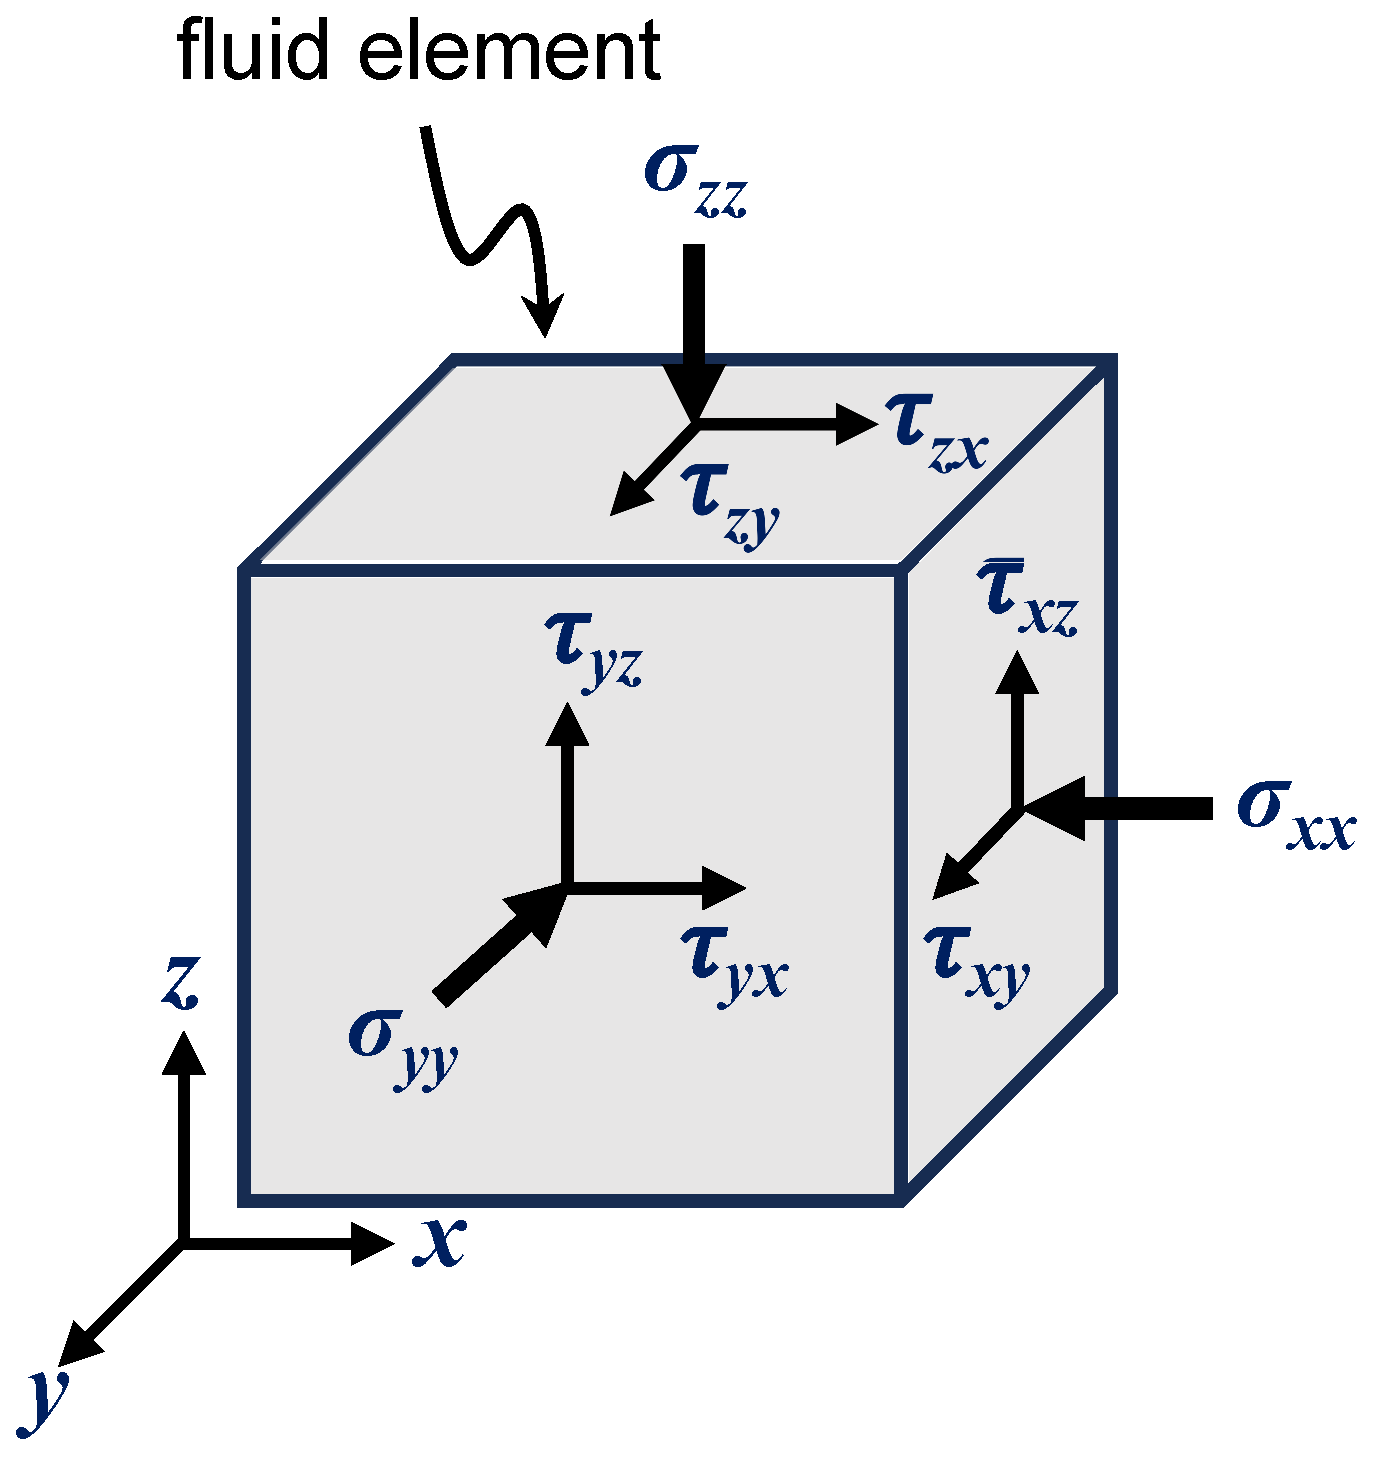
\includegraphics[width=\textwidth]{img/stress_tensor.eps}
\end{minipage}

\begin{enumerate}\setcounter{enumi}{2}
    \item The \textbf{deviatoric} (\textit{a.k.a.} dynamic or viscous) stress raises when a fluid body is in motion. It can be approximated as a linear function of the rate of strain,
    \[
        d_{ij} = \mathcal{C}_{ijkl} \ \frac{\partial}{\partial t} \bigg( \frac{\partial X}{\partial x} \bigg).
    \]
    where $\mathcal{C}_{ijkl}$ is a 4\textsuperscript{th}-order tensor {\color{gray}(treat this as the coefficients in a linear function?)}. $X$ is the initial (`reference') configuration. Moreover, the rate of strain is equivalent to the velocity gradient,
    \[
        \frac{\partial}{\partial t} \bigg( \frac{\partial X}{\partial x} \bigg) = \underbrace{\frac{\partial}{\partial x} \bigg( \frac{\partial X}{\partial t} \bigg)}_{\nabla \mathbf{u}} 
        \quad \Longrightarrow \quad 
        d_{ij} = \mathcal{C}_{ijkl} \nabla \mathbf{u} = \mathcal{C}_{ijkl} \ \frac{1}{2} \bigg[ \bigg(\frac{\partial u_{i}}{\partial x_{j}} + \frac{\partial u_{j}}{\partial x_{i}}\bigg) + \cancelto{0,\ \text{neglect rotation}}{\bigg(\frac{\partial u_{i}}{\partial x_{j}} - \frac{\partial u_{j}}{\partial x_{i}}\bigg)} \bigg].
    \]
    Under \textit{various} assumptions (material isotropy, tensor symmetry, and major symmetry), the number of combinations of $\mathbb{C}_{ijkl}$ can be reduced from 3\textsuperscript{4}=81 {\color{gray}(4 free indices, each ranges 1-3)} to 2. We have
    \[
        \mathcal{C}_{ijkl} = \lambda \delta_{ij} \delta_{kl} + \mu (\delta_{jk} \delta_{il} + \delta_{ik} \delta_{jl} ),
    \]
    where $\lambda$ and $\mu$ are the bulk viscosity {\color{gray}(less significant, especially for incompressible fluid)} and dynamics viscosity {\color{gray}(more significant)}, respectively. To put all the facts together, the deviatoric stress
    \begin{align*}
        d_{ij}
        & = \lambda \delta_{ij} \delta_{kl} + \mu (\delta_{jk} \delta_{il} + \delta_{ik} \delta_{jl} ) \times \bigg[ \frac{1}{2} \bigg(\frac{\partial u_{i}}{\partial x_{j}} + \frac{\partial u_{j}}{\partial x_{i}}\bigg) \bigg] \\
        & = \lambda \delta_{ij} \underbrace{\frac{\partial u_{k}}{\partial x_{k}}}_{\nabla \cdot \mathbf{u}} + \mu \underbrace{\bigg(\frac{\partial u_{i}}{\partial x_{j}} + \frac{\partial u_{j}}{\partial x_{i}}\bigg)}_{\text{strain rate}, \ 2\mathbf{e}}.
    \end{align*}
\end{enumerate}

\subsection{Strain Rate Tensor}
\begin{table}[H]
    \centering
    \begin{tabular}{c|c}
    \toprule
    \multicolumn{2}{c}{Strain rate: $\mathbf{e} = \frac{1}{2}\bigg(\frac{\partial u_{i}}{\partial x_{j}} + \frac{\partial u_{j}}{\partial x_{i}}\bigg)=\frac{1}{2}(\nabla \mathbf{u}+(\nabla \mathbf{u})^\top)$} \\
    \toprule
    in Cartesian coord. sys. & in cylindrical coord. sys. \\
    \midrule
    $
    \begin{pmatrix}
      \frac{\partial u}{\partial x} & \frac{1}{2}(\frac{\partial u}{\partial y}+\frac{\partial v}{\partial x}) & \frac{1}{2}(\frac{\partial u}{\partial z}+\frac{\partial w}{\partial x})\\[0.8em]
      
      \frac{1}{2}(\frac{\partial u}{\partial y}+\frac{\partial v}{\partial x}) & \frac{\partial v}{\partial y}  & \frac{1}{2}(\frac{\partial v}{\partial z}+\frac{\partial w}{\partial y})\\[0.8em]
      
      \frac{1}{2}(\frac{\partial u}{\partial z}+\frac{\partial w}{\partial x}) & \frac{1}{2}(\frac{\partial v}{\partial z}+\frac{\partial w}{\partial y})  & \frac{\partial w}{\partial z}\\
    \end{pmatrix}
    $
    & 
    $
    \begin{pmatrix}
      \frac{\partial u_{r}}{\partial r} & \frac{1}{2}(r\frac{\partial (u_{\theta}/r)}{\partial r}+\frac{1}{r}\frac{\partial u_{r}}{\partial \theta}) & \frac{1}{2}(\frac{\partial u_{z}}{\partial r}+\frac{\partial u_{r}}{\partial z})\\[0.8em]
      
      \frac{1}{2}(r\frac{\partial (u_{\theta}/r)}{\partial r}+\frac{1}{r}\frac{\partial u_{r}}{\partial \theta}) & \frac{1}{r}\frac{\partial u_{\theta}}{\partial \theta}+\frac{u_{r}}{r} & \frac{1}{2}(\frac{\partial u_{\theta}}{\partial z}+\frac{1}{r}\frac{\partial u_{z}}{\partial \theta})\\[0.8em]
      
      \frac{1}{2}(\frac{\partial u_{z}}{\partial r}+\frac{\partial u_{r}}{\partial z}) & \frac{1}{2}(\frac{\partial u_{\theta}}{\partial z}+\frac{1}{r}\frac{\partial u_{z}}{\partial \theta})  & \frac{\partial u_{z}}{\partial z}\\
    \end{pmatrix}
    $ \\
    \bottomrule
    \end{tabular}
\end{table}


\subsection{Incompressible Fluid Constitutive Relationship}
\vspace{-.2cm}
To put up all things together, the Cauchy stress tensor is
\begin{align*}
    \sigma_{ij} 
    & = -p\delta_{ij} + d_{ij} \\
    & = -p\delta_{ij} + \lambda \delta_{ij} \frac{\partial u_{k}}{\partial x_{k}}+ \mu \bigg(\frac{\partial u_{i}}{\partial x_{j}} + \frac{\partial u_{j}}{\partial x_{i}}\bigg) \\
    & = -p\mathbf{I} + \lambda (\nabla \cdot \mathbf{u})\mathbf{I} + 2\mu \mathbf{e}.
\end{align*}

\paragraph{Cauchy's Equation} For the incompressible fluid, $\dfrac{\partial u_k}{\partial x_k} = 0$ (mass conservation). Hence, $\displaystyle \sigma_{ij} = -p\delta_{ij} + \mu \bigg(\frac{\partial u_{i}}{\partial x_{j}} + \frac{\partial u_{j}}{\partial x_{i}}\bigg)$. \\

Cauchy's equation is obtained by equating the total forces acting on a fluid element to its acceleration, based on Newton's 2\textsuperscript{nd} Law: $\mathbf{F} = m \mathbf{a}$.
\[  
    \underbrace{\rho \frac{D\mathbf{u}}{D t} }_{m \times \mathbf{a}} 
    \quad = \quad
    \underbrace{\nabla \cdot \boldsymbol{\sigma} + \rho \mathbf{f}}_{\mathbf{F}_{\rm internal} \ + \ \mathbf{F}_{\rm external}}, 
\]
where $\displaystyle \frac{D\mathbf{u}}{D t} = \frac{\partial \mathbf{u}}{\partial t} + \mathbf{u} \cdot \nabla \mathbf{u}$ is the material derivative. By expanding  $\frac{D\mathbf{u}}{D t}$ and $\nabla \cdot \boldsymbol{\sigma}$, we will obtain the celebrated Navier-Stokes equation, which depicts the conservation of linear momentum.


\vfill
{\small \color{gray}Drafted by B. Li, H. El Nashar, and C. H. Yap,  \today}
% %% TITLE	Physiological Fluid Mechanics, last page

%% DATE		- Nov 19, 2023     create

%% AUTHOR	BINGHUAN W LI (Dept. Chemical Eng/Bio Eng, Imperial)
%%          PETER Y XIE (Dept. Mech Eng, Stanford)

%% compiled in XeLaTeX with Tex Live version 2023.

%% This work is licensed under a Creative Commons Attribution-NonCommercial 4.0 International License.

\newpage
\thispagestyle{empty}
\newgeometry{margin=1.8cm}

\mbox{}
\vfill    
\begin{figure}[H]
    \includegraphics[right]{img/by-nc.eps}
\end{figure}
\textit{This work is licensed under a Creative Commons Attribution-NonCommercial 4.0 International License.}

\end{document}